\section{URDAD}

\begin{frame}{URDAD}
   \begin{itemize} 
    \item Systematic methodology for technology-neutral A\&D
		\begin{itemize}
		  \item service-oriented approach
		  \item generates MDA's PIM
		\end{itemize}
   \end{itemize}

  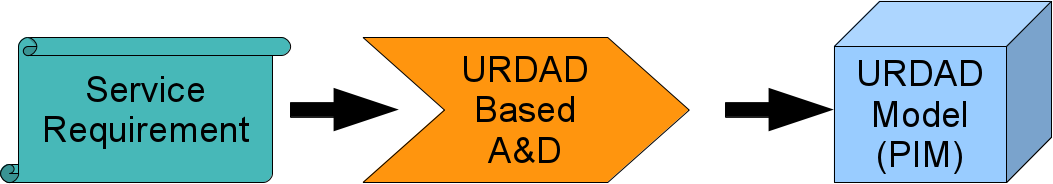
\includegraphics[width=100mm]{urdadHighLevel}
\end{frame}


%---------------------------------------%

\begin{frame}[fragile]
  \frametitle{URDAD as recursive analysis \& design algorithm}

\lstset{language=pseudoCode}
\begin{lstlisting}[numbers=left,escapechar=|]
class Urdad
{
  provideService(serviceRequirement):Service
  {
    serviceContract = negotiateContract(serviceRequirement)
 
    try
    {
      return serviceRegistry.getService(serviceContract)
    }
    catch (noRealizingServiceException)
    {
      service = designService(serviceContract)

      for (lowerLevelServiceRequirement : service.requiredServices)
\end{lstlisting}
\vspace{-\baselineskip}
\begin{lstlisting}[backgroundcolor=\color{pink}]
        provideService(lowerLevelServiceRequirement)
\end{lstlisting}
\vspace{-\baselineskip}
\begin{lstlisting}
    }
  }
}
\end{lstlisting}
\end{frame}

%---------------------------------------%

\begin{frame}[fragile]
  \frametitle{URDAD analysis phase}
\lstset{language=pseudoCode}
\begin{lstlisting}[numbers=left,escapechar=|]
class UrdadAnalysis
{
  negotiateContract(serviceRequirement):ServiceContract
  {
    for (stakeholder:identifyStakeHolders(serviceRequirement))
    {
      functionalRequirements = sourceFunctionalRequirements(stakeholder, serviceRequirement)
      qualityRequirements = sourceFunctionalRequirements(stakeholder, serviceRequirement)
    }
    negotiateConsistentRequirements()
    groupFunctionalRequirementsIntoServiceRequirements(functionalRequirements)
    for (functionalRequirement:functionalRequirements)
      defineCondition(functionalRequirement)
        // includes test & associated exception
    specifyDatastructuresForRequestAndResultClasses()
    assembleServiceContract()
    assignServiceContractToResponsibilityDomain()
    return serviceContract
  }
}
\end{lstlisting}
\end{frame}
